\chapter{Основные компоненты системы}

\section{Основные структуры данных}

\subsection{Структура camera}
\begin{verbatim}
struct camera {
    /*--- Поля, заполняются данными из БД ---*/
    int id;
    char *url;
    char *name;
    int analize_frames;
    int threshold;
    int motion_delay;
    /*-------------------------*/
    
    // Выставляется = 0 при завершении работы сервера
    int active;
    
    /*--- Структуры ffmpeg ---*/
    AVFormatContext *context;
    AVCodecContext  *codec;
    AVStream        *input_stream;
    AVFormatContext *output_context;
    AVStream        *output_stream;
    AVIOInterruptCB int_cb;
    int video_stream_index;
    /*-------------------------*/

    /*--- Информация о файле, в который производится запись ---*/
    int file_id; // ID файла в таблице videofiles
    time_t file_started_at; // время начала записи файла
    /*-------------------------*/
    
    // время получения крайнего пакета данных от камеры
    time_t last_io;
    // время крайнего обновления картинки для показа в UI
    time_t last_screenshot;
	// список <<подписанных>> на изображение с камеры потребителей
    l1* cam_consumers_list;
};
\end{verbatim}

Cтруктура описывает камеру.

\subsection{Структура screen}
\begin{verbatim}
struct screen {
    int type; // ARCHIVE или REAL
    int ncams; // количество камер, интересующих пользователя
    struct camera **cams;
    unsigned int session_id; // ID RTSP сессии
    time_t timestamp; // момент времени, интересующий пользователя
    
    /*--- Структуры ffmpeg и RTSP сервера,
          отвечающие, за доставку видео клиенту ---*/
    GstRTSPMediaFactory *factory;
    AVFormatContext *rtp_context;
    AVStream *rtp_stream;
    int rtp_port;
    /*-------------------------*/
    
    /*--- Поля используются, если количество камер больше 1 ---*/
    uint8_t *frame; // буфер для изображения
    // количество камер, которые еще не скопировали изображение в буфер
    int left_cameras;
    pthread_mutex_t counter_lock; // мьютекс для синхронизации
    /*-------------------------*/
};
\end{verbatim}

Структура $screen$ используется при показе видео пользователю.
Она хранит информацию об интересующих пользователя камерах.

\subsection{Структура cam\_consumer}
\begin{verbatim}
struct cam_consumer {
    struct screen *screen;
    int position;
};
\end{verbatim}

Описывает <<потребителя>> изображения с камеры.
Поле $position$ определяет местонахождение изображения с данной камеры в сводной картинке.

\section{Модуль работы с конфигурационным файлом и базой данных}

С помощью библиотеки libconfig из конфигурационного файла считываются основные настройки системы:
адрес в файловой системе для хранения архива видеозаписей,
реквизиты базы данных(сетевой адрес и порт, имя пользователя и пароль, название схемы).

Пример конфигурационного файла:
\begin{verbatim}
	db_host: "localhost"
	db_port: "5432"
	db_name: "cameras"
	db_login: "cameras"
	db_password: "password"
	store_dir: "/storage"
\end{verbatim}

После чтения конфигурационного файла создается соединение с базой данных.
Используется библиотека libpq.
Модуль содержит функции, требующие обращения к базе данных.
Функции производят формирование SQL-запросов и обработку результатов.

При запуске сервера модуль осуществляет соединение с базой данных (функция $init\_pg\_conn$),
получает из таблицы $cameras$ записи о камерах и инициализирует структуры $camera$
(функция $select\_cameras$). После этого для каждой камеры создается поток $pthread$,
производящий запись видео.

\section{Модуль записи видео}
Используются библиотеки ffmpeg.
Модуль устанавливает соединения со всеми камерами, инициализирует структуры ffmpeg для
чтения видеопотока и для записи его в файл. В цикле программа получает кадры от камеры, при
необходимости декодирует кадры и передает их для анализа в модуль обнаружения движения
или в модуль показа изображений с камер пользователю.

Через заданный период времени программа закрывает записываемый файл и открывает новый.
Файлы размещаются в директории для хранения архива видеозаписей по адресу,
который формируется по следующему правилу:

\begin{verbatim}
/адрес_видео_архива/код_камеры/yyyymmdd/yyyyymmddHHMMSS.h264
\end{verbatim}

Блоки yyyymmdd и yyyyymmddHHMMSS~--- форматы даты начала записи.
Например, если архив видео находится в /storage/, код камеры cam\_1 и запись началась
01.02.13 в 23:55:32, то файл будет расположен по адресу:

\begin{verbatim}
/storage/cam_1/20130201)/20130201235532.h264
\end{verbatim}

Информация о созданных файлах сохраняется в базу данных.
Записываются ID камеры, время начала и окончания записи.
Данная информация позволяет сопоставить интересующий пользователя момент времени
с видеофайлом, хранящим кадры, относящиеся к данному моменту.

Видеопоток изначально сохраняется в формат h264 и не упаковывается в контейнер, чтобы была
возможность просмотреть незавершенный файл. После окончания записи в файл, видеопоток
упаковывается в контейнер mp4. Меняется расширение файла с h264 на mp4 и в базе данных
у записи, относящейся к данному файлу, делается пометка~--- поле $mp4$ выставляется
в $true$.

Такая последовательность действий необходима, т.к. в случае сохранения потока сразу в
контейнер mp4, становится невозможно прочитать недавно записанные данные до тех пор,
пока файл не будет закрыт и вся служебная информация будет записана в контейнер.
Хранение видеозаписей в формате h264 также создает ряд неудобств, т.к. чистые видеоданные не
содержат информации о видеопотоке (например количество кадров в секунду,
продолжительность записи). Это затрудняет открытие видеофайла в стандартном видеоплеере~---
видеофайлы или не открываются или проигрываются с неправильной скоростью.
Также становится невозможным быстрый поиск по видеофайлу~--- для того, чтобы начать чтение
с произвольного момента времени, необходимо прочитать весь поток до этого момента.

Раз в минуту обновляется картинка (кадр с камеры) для показа в интерфейсе пользователя.

В случае остановки сервера, модуль совершает корректное закрытие файлов и соединений,
производит освобождение ресурсов.

\section{Модуль обнаружения движения}
Кадры с камеры поступают от модуля видеозаписи.
Они преобразуются в изображения в оттенках серого.

Перед обработкой кадров с помощью функций OpenCV нужно преобразовать структуры данных ffmpeg
в структуры данных OpenCV.

Обнаружение движения происходит следующим образом.
Текущий кадр попиксельно вычитается из предыдущего с помощью функции cvAbsDiff.
Результирующая картинка проходит пороговое преобразование с помощьюфункции cvThreshold.
Это позволяет отсеять шумы изображения и исключить ложное срабатывание.
Чувствительность данного фильтра можно настроить в интерфейсе пользователя.
Далее подсчитывается количество пикселей, прошедших через фильтр.
Если их количество больше 1\% от общего количества пикселов в изображении,
то можно говорить о наличии движения.

Следует отметить, что это один из возможных алгоритмов обнаружения движения.
Он прост, но при этом эффективен. Данный способ описан в статье \cite{motion_detection}.

На рисунках \ref{motion_detection_1}, \ref{motion_detection_2}, \ref{motion_detection_3}
приведен пример работы алгоритма по обнаружению движения.

\begin{figure}[!htb]
\minipage{0.49\textwidth}
	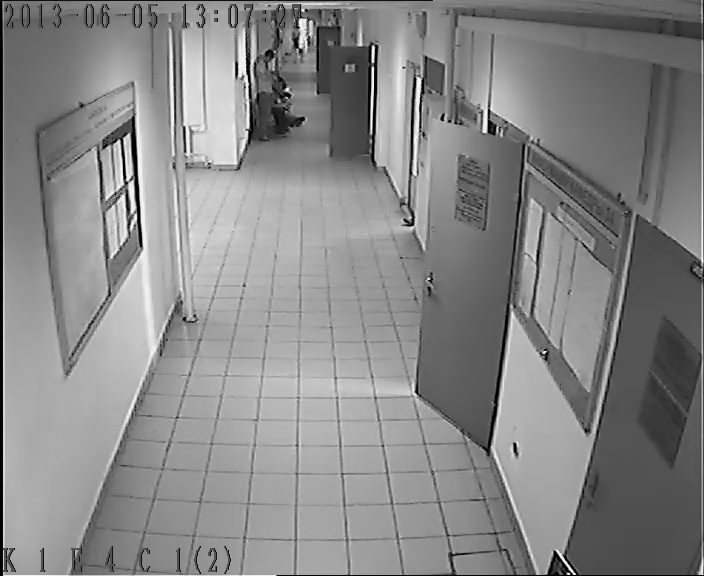
\includegraphics[width=\linewidth]{img/frame_1.png}
	\caption{Кадр 1}
	\label{motion_detection_1}
\endminipage\hfill
\minipage{0.49\textwidth}
	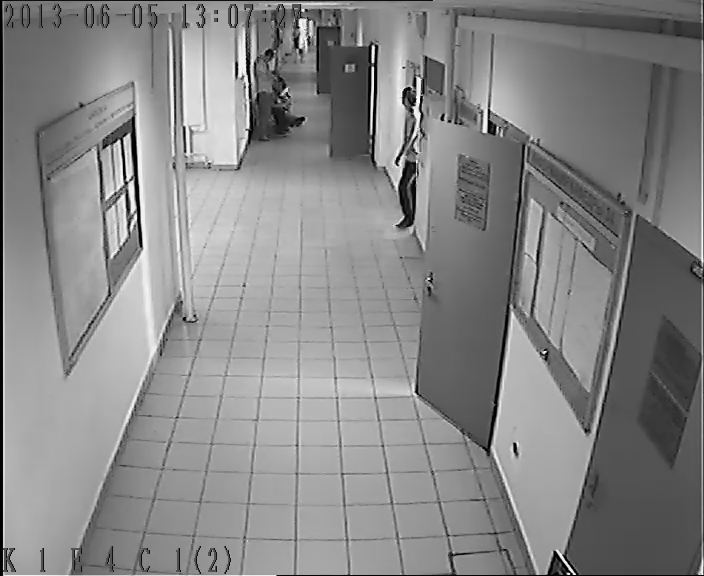
\includegraphics[width=\linewidth]{img/frame_2.png}
	\caption{Кадр 2}
	\label{motion_detection_2}
\endminipage

\def\svgwidth{\columnwidth}
\center{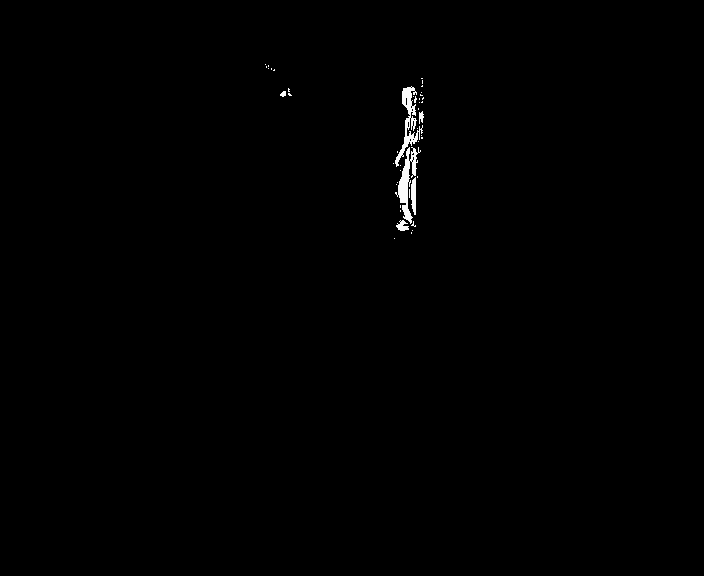
\includegraphics[width=0.5\linewidth]{img/silh.png}}
\caption{Разница между кадрами}
\label{motion_detection_3}
\end{figure}


\section{Модуль взаимодействия с графическим интерфейсом}
Для взаимодействия с графическим интерфейсом пользователя сервер открывает unix сокет
по адресу $/tmp/videoserver$. Модуль осуществляет получение команд, их интерпретацию и исполнение.
Команды поступают в формате json. Парсинг json осуществляется при помощи библиотеки json-parser
\cite{json_parser}.

Модуль представляет из себя однопоточный неблокирующий сервер. Данное требование необходимо, т.к.
графический интерфейс существует отдельно от видеосервера, может перезапускаться или запускаться в
нескольких экземплярах. При этом каждый экземпляр устанавливает с видеосервером отдельное соединение.
Сервер использует системный вызов $poll$ и устанавливает всем сокетам флаг O\_NONBLOCK.
При разработке использовалась документация IBM по неблокирующим сокетам \cite{socket_doc}.

Общение происходит по синхронному протоколу. При этом клиент всегда инициализирует запрос.
Видеосервер производит необходимые действия и отвечает строкой с данными в формате JSON.
Пустая строка означает окончание ответа или запроса.

Серверу могут поступать следующие виды команд:
\smallskip
\begin{itemize}
	\item запрос на трансляцию видео с камер или из архива;
	\item запрос информации о видеокамере;
	\item запрос информации о состоянии сервера и файлового хранилища.
\end{itemize}

\section{Модуль трансляции видео}
Модуль необходим, чтобы передавать пользователю видеозапись интересующих его моментов архива или
живую картинку с одной, четырех, девяти или шестнадцати камер.
Для этих целей используется библиотека gst-rtsp-server. Для своей работы она использует набор
мультимедийных библиотек Gstreamer.

В отдельном потоке запускается RTSP сервер, способный обслуживать несколько одновременных соединений,
при этом показывая пользователям различные потоки.
Сервер допускает динамическую конфигурацию, т. е. возможность во время работы сервера добавлять
и удалять каналы.

Возможны 3 ситуации, определяющие как будет работать сервер при показе видео пользователю.
\begin{enumerate}
	\item Пользователь хочет посмотреть живое изображение с одной камеры.
	\item Пользователь хочет одновременно посмотреть живое изображение с нескольких камер.
	\item Пользователь хочет посмотреть видео из архива.
\end{enumerate}

В первом случае в список $cam\_consumers\_list$ интересующей видеокамеры добавляется новая запись
$cam\_consumer$, и при получении кадров от камеры они одновременно и сохраняются в файл и отправляются
пользователю для просмотра.

Во всех случаях создается RTP поток, который забирается RTSP сервером и передается пользователю.

Т.к. каждый пользователь единолично просматривает один поток, то после завершения просмотра
(отправка RTSP серверу команды стоп или по таймауту в случае разрыва соединения) RTSP сервер
должен закончить обслуживание канала.
Также должно быть завершено создание видеопотока со стороны видеосервера.
Для этих целей сервер периодически (каждые 3 секунды) проверяет, что у всех поставщиков
видеоданных есть свои потребители. Поставщики видеоданных описываются структурой $screen$.

\section{Модуль показа архива}
В случае, если пользователя интересует архивная видеозапись, сервер определяет, в каком файле
находится интересующий его момент. Этот файл открывается и запускается новый поток, читающий видео
поток из файла и передающий его пользователю. В случае окончания файла ищется файл-продолжение,
предыдущий файл закрывается, а вещание продолжается из следующего файла.

Возможны две ситуации в работе данного модуля:

\begin{itemize}
 \item запись в видеофайл завершена и данные упакованы в контейнер mp4;
 \item запись видеоданных продолжается в формате h264.
\end{itemize}

В первом случае файл открывается по стандартному для библиотеки libavformat сценарию.
Во втором случае необходимо явно указать, что в файле находятся видеоданные, закодированные
кодеком h264. Также необходимо узнать количество кадров в секунду для корректного
воспроизведения файла. Эта информация есть в структуре $AVStream$, которая хранится
в дескрипторе видеокамеры (структура $camera$). Т.к. быстрый поиск в видеофайле в формате h264
невозможен (например, используя функцию $av\_seek\_frame$), приходится считывать все кадры до
интересующего момента. Зная количество кадров в секунду и время до необходимого момента, можно
вычислить, сколько кадров нужно пропустить.

Далее кадры читаются со скоростью нормального воспроизведения файла и отправляются пользователю.
Для поддержания скорости отправки кадров используется системный вызов $usleep$.

%\section{Модуль показа изображения с нескольких камер}

\section{Модуль слежения за объемом дискового пространства}
Главный поток программы устанавливает таймер, по которому вызывается функция проверки объема дискового
пространства. В случае, если остается менее 1ГБ дискового пространства, выбираются архивные видеозаписи
суммарным размером не менее 200МБ. В базе данных помечается, что эти файлы были удалены, после чего они
стираются из файловой системы.

\section{Графический интерфейс пользователя}
Графический интерфейс пользователя предоставляется посредством web-приложения, созданного на базе
фреймворка Ruby on Rails. Интерфейс позволяет управлять камерами, просматривать архив и
живую картинку с выбранных камер. Интерфейс является кросплатформенным. Для работы с настройками
сервера и камер необходим любой веб-браузер. Для просмотра видео требуется наличие в
браузере плагина VLC.
Эталоном был выбран браузер Mozilla Firefox с плагином VLC.

\section{Структура базы данных }
Ключевые таблицы базы данных.

\subsection{Таблица cameras}
Хранит информацию о камерах и настройках для каждой из них.

\begin{center}
\begin{tabular}{ | l | l | p{11cm} |}
\hline
code & string & Краткое название для камеры. Также является названием директории, в которой хранятся видеозаписи с данной камеры. \\ \hline
about & string & Описание камеры. \\ \hline
url & string & Сетевой адрес камеры. \\ \hline
analize\_frames & integer & Интервал в кадрах между проведением анализа на наличие движения. \\ \hline
threshold & integer & Пороговое значение для фильтра шума \\ \hline
motion\_delay & integer & Время в секундах, по прошествии которого в случае отсутствия движения предыдущие срабатывания детектора движения считаются отдельным событием. Если между срабатываниями детектора движения проходит менее motion\_delay секунд, эти срабатывания будут относиться к одному событию. \\ \hline
\end{tabular}
\end{center}

\subsection{Таблица events}
Хранит информацию о произошедших событиях.

\begin{center}
\begin{tabular}{ | l | l | p{11cm} |}
\hline
camera\_id & integer & идентификатор камеры в таблице cameras \\ \hline
started\_at & datetime & время начала события \\ \hline
finished\_at & datetime & время завершения события \\ \hline
\end{tabular}
\end{center}

\subsection{Таблица videofiles}
Хранит информацию о всех записанных видеофайлах.

\begin{center}
\begin{tabular}{ | l | l | p{11cm} |}
\hline
camera\_id & integer & идентификатор камеры в таблице cameras \\ \hline
started\_at & datetime & время начала записи \\ \hline
finished\_at & datetime & время завершения записи \\ \hline
deleted\_at & datetime & время, когда файл был удален в результате очистки архива \\ \hline
mp4 & boolean & был ли видеопоток упакован в контейнер mp4 \\ \hline
\end{tabular}
\end{center}
